\chapter{Recurrent Nets}
% Authors: Qintai Liu
% Lecture date: 3/11/2019

\section{Simple Recurrent Net}
% Authors: Qintai Liu
% Lecture date: 3/11/2019

The idea behind RNNs is to make use of sequential information. 
In a traditional neural network we assume that all inputs are independent of each other.
But for many tasks that’s a very bad idea. 
If you want to predict the next word in a sentence you better know which words came before it. 
RNNs are called recurrent because they perform the same task for every element of a sequence, with the output being depended on the previous computations. 
Another way to think about RNNs is that they have a “memory” which captures information about what has been calculated so far. 
In theory RNNs can make use of information in arbitrarily long sequences, but in practice they are limited to looking back only a few steps. 
Here is what a typical RNN looks like:\cref{fig:param}

\begin{figure}[h]
    \centering
    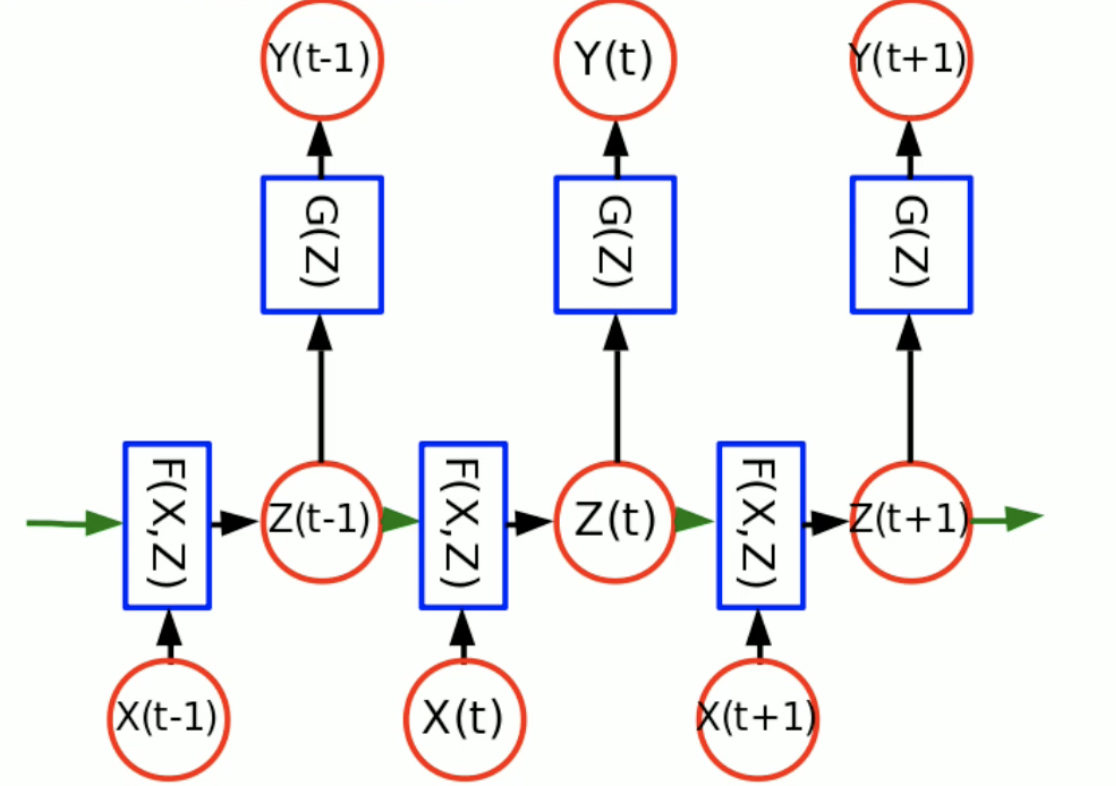
\includegraphics[width=150pt]{lectures/06-b-rnn/image/rnn.png}
    \caption{Simple Recurrent Net}
    \label{fig:Simple RNN}
\end{figure}

\begin{itemize}
  \item $x_{t}$ is the input at time step $t$
  \item $z_{t}$ is the hidden state at time $t$. $z_{t}$ is calculated based on the input at the current step and the previous hidden state:
  $z_t = F(x_t, z_{t-1})$
  \item $y_t$ is the output at step $t$. $y_t = G(z_t)$
\end{itemize}



\section{Issue of Simple Recurrent Net}
% Authors: Qintai Liu
% Lecture date: 3/11/2019
\subsection{Backpropagation Through Time}
% Authors: Qintai Liu
% Lecture date: 3/11/2019
In order to know the issue of simple RNN, we first need to know how the gradient is calculated in terms of RNN. Suppose the hidden state($z_t$) is calculated as below:

\[\bar{z_t} = W_X x_t + W_Z z_{t-1}\]
\[z_t = f(\bar{z_t})\]
\[y_t = g(z_t)\]

To measures the effect of the $(t-n)$-th input symbot $x_{t-n}$, where $n\leq{t}$, on the $t$-th hidden state $z_t$ of the simple recurrent neural network, we need to calculate the derivative shown below
\[\frac{\partial z_t}{\partial x_{t-n}}=\frac{\partial z_t}{\partial z_{t-n}}\frac{\partial z_{t-n}}{\partial \bar{z}_{t-n}}\frac{\partial \bar{z}_{t-n}}{\partial x_{t-n}}\]

Among these three terms in the right hand side of the above equation, we will focus on the first term

\begin{equation} \label{eq:bptt}
\frac{\partial z_t}{\partial z_{t-n}} = (\underbrace{\frac{\partial z_t}{\partial \bar{z}_{t}}}_{a}\underbrace{\frac{\partial \bar{z}_{t}}{\partial z_{t-1}}}_{b})
(\underbrace{\frac{\partial z_{t-1}}{\partial \bar{z}_{t-1}}}_{a}\underbrace{\frac{\partial \bar{z}_{t-1}}{\partial z_{t-2}}}_{b}) \ldots 
(\underbrace{\frac{\partial z_{t-n+1}}{\partial \bar{z}_{t-n+1}}}_{a}\underbrace{\frac{\partial \bar{z}_{t-n+1}}{\partial z_{t-n}}}_{b})
\end{equation}

First, consider \cref{eq:bptt}(a), which is the derivative of a nonlinear activation function used in the simple recurrent neural network.

Next, we look at \cref{eq:bptt}(b). We know

\[\frac{\partial \bar{z}_{t}}{\partial z_{t-1}} = W_Z\]

From these two, we get
\begin{align} \label{eq:bptt_result}
\begin{split}
\frac{\partial z_t}{\partial z_{t-n}} &= (\frac{\partial z_t}{\partial \bar{z}_{t}}\frac{\partial \bar{z}_{t}}{\partial z_{t-1}})
(\frac{\partial z_{t-1}}{\partial \bar{z}_{t-1}}\frac{\partial \bar{z}_{t-1}}{\partial z_{t-2}}) \ldots 
(\frac{\partial z_{t-n+1}}{\partial \bar{z}_{t-n+1}}\frac{\partial \bar{z}_{t-n+1}}{\partial z_{t-n}}) \\
&= (\frac{\partial z_t}{\partial \bar{z}_{t}}W_Z)
(\frac{\partial z_{t-1}}{\partial \bar{z}_{t-1}}W_Z) \ldots 
(\frac{\partial z_{t-n+1}}{\partial \bar{z}_{t-n+1}}W_Z) \\
&= \prod\limits_{i=t-n+1}^{t} (\frac{\partial z_i}{\partial \bar{z}_{i}}W_Z)
\end{split}
\end{align}

Suppose the recurrent activation function $f$ is linear, \cref{eq:bptt_result} reduces to
\begin{equation} \label{eq:bptt_linear_result}
\frac{\partial z_t}{\partial z_{t-n}} = W_Z^{n-1}
\end{equation}


\subsection{Exploding Gradients}
% Authors: Qintai Liu
% Lecture date: 3/11/2019
In recurrent neural networks, gradients can accumulate during an update and result in very large gradients. 
These in turn result in large updates to the network weights, and in turn, an unstable network. 
At an extreme, the values of weights can become so large as to overflow and result in NaN values.

The explosion occurs through exponential growth by repeatedly multiplying gradients through the network layers that have values larger than $1.0$.

From \cref{eq:bptt_linear_result}, $\frac{\partial z_t}{\partial z_{t-n}}$ will likely explode as $n \rightarrow \inf$ if $e_{max} > 1$, where $e_{max}$ is the largest eigenvalue of $W_Z$.

\subsection{Vanishing Gradients}
% Authors: Qintai Liu
% Lecture date: 3/11/2019
When we do Back-propagation in the recurrent neural networks and calculating gradients of loss with respect to the weights , the gradients may also get smaller and smaller as we keep on moving backward in the Network. 
This means that the neurons in the earlier layers learn very slowly as compared to the neurons in the later layers in the hierarchy. 
The earlier layers in the network are slowest to train.

From \cref{eq:bptt_linear_result}, $\norm{\frac{\partial z_t}{\partial z_{t-n}}} \rightarrow 0$ when $e_{max} < 1$, where $e_{max}$ is the largest eigenvalue of $W_Z$.

\section{Gradient clipping}
% Authors: Qintai Liu
% Lecture date: 3/11/2019
Fortunately it's easy to solve the problem of exploding gradients by doing gradient clipping.
First, it is straightforward to detect whether the exploding gradient happened by inspecting the norm of the gradient for the cost with respect to the parameters $\norm{\nabla}$.
If the gradient's norm is larger than some predefined threshold $\tau > 0$, we can renormalize the norm of the gradient to be $\tau$.

\[
\widetilde{\nabla}=\left\{
            \begin{array}{ll}
              \tau\frac{\nabla}{\norm{\nabla}} & \text{if}  \norm{\nabla}>\tau\\
              \nabla & \text{otherwise}
            \end{array}
          \right.
\]

\section{Long Short-Term Memory}
% Authors: Qintai Liu
% Lecture date: 3/11/2019

\begin{figure}[h]
  \centering
      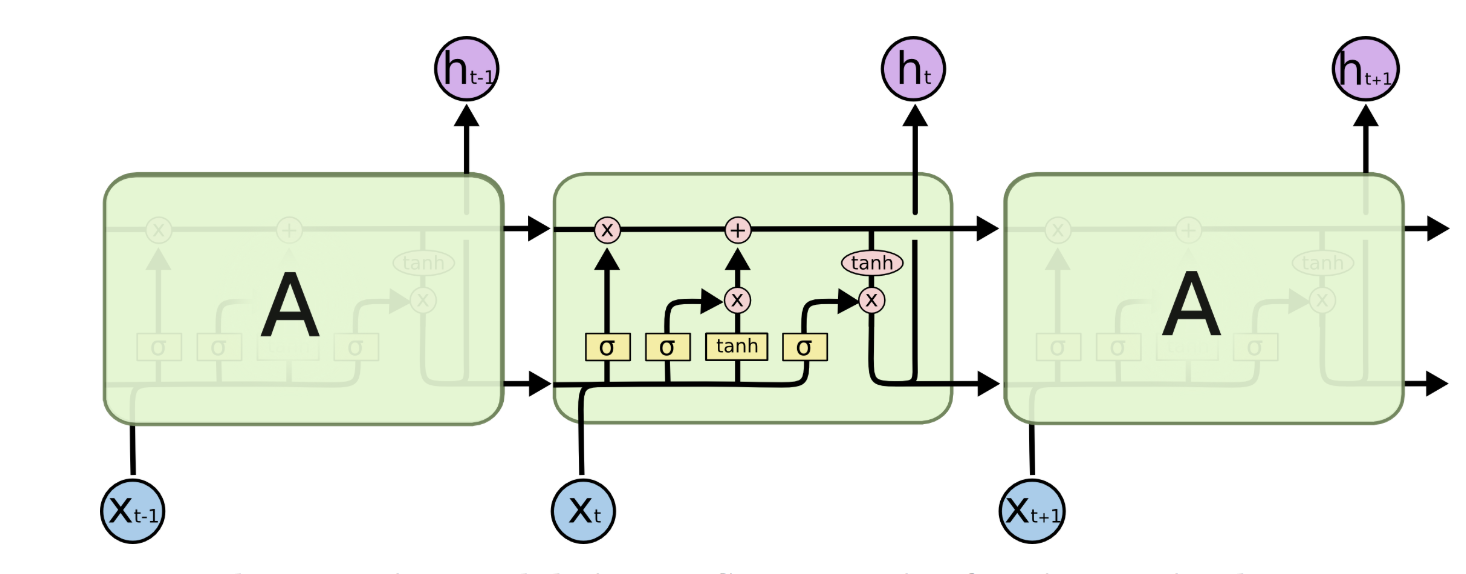
\includegraphics[width=0.8\textwidth,height=4.5cm]{lectures/06-b-rnn/image/lstm.png}
          \caption{
            The repeating module in an LSTM contains four interacting layers.
            \href{http://colah.github.io/posts/2015-08-Understanding-LSTMs/}{Source}
          }
          \label{fig:lstm}
\end{figure}

Long Short Term Memory networks – usually just called “LSTMs” – are a special kind of RNN, capable of learning long-term dependencies. 
They were introduced by Hochreiter \& Schmidhuber (1997). They work tremendously well on a large variety of problems, and are now widely used.
LSTMs are explicitly designed to avoid the long-term dependency problem. 
Remembering information for long periods of time is practically their default behavior, not something they struggle to learn!

The forget gate in LSTM is to decide what information we’re going to throw away from the cell state.
\[f_t = \sigma(W_{fh}h_{t-1}+W_{fx}x_t + b_f) \]

Input gate decides which values we’ll update
\[i_t = \sigma(W_{ih}h_{t-1} + W_{ix}x_t + b_i)\]

New candidate cell state is to decide what new information we’re going to store in the cell state.
\[\widetilde{c}_t = tanh(W_{ch}h_{t-1} + W_{cx}x_t + b_c)\]

New cell state:
\[c_t = f_t*c_{t-1} + i_t*\widetilde{c}_t\]

Output Gate decides what parts of the cell state we’re going to output.
\[o_t = \sigma(W_{oh}h_{t-1} + W_{ox}x_t + b_o)\]

Output:
\[h_t = o_t*tanh(c_t)\]

\section{Gated Recurrent Units}
% Authors: Qintai Liu
% Lecture date: 3/11/2019

\begin{figure}[h]
  \centering
      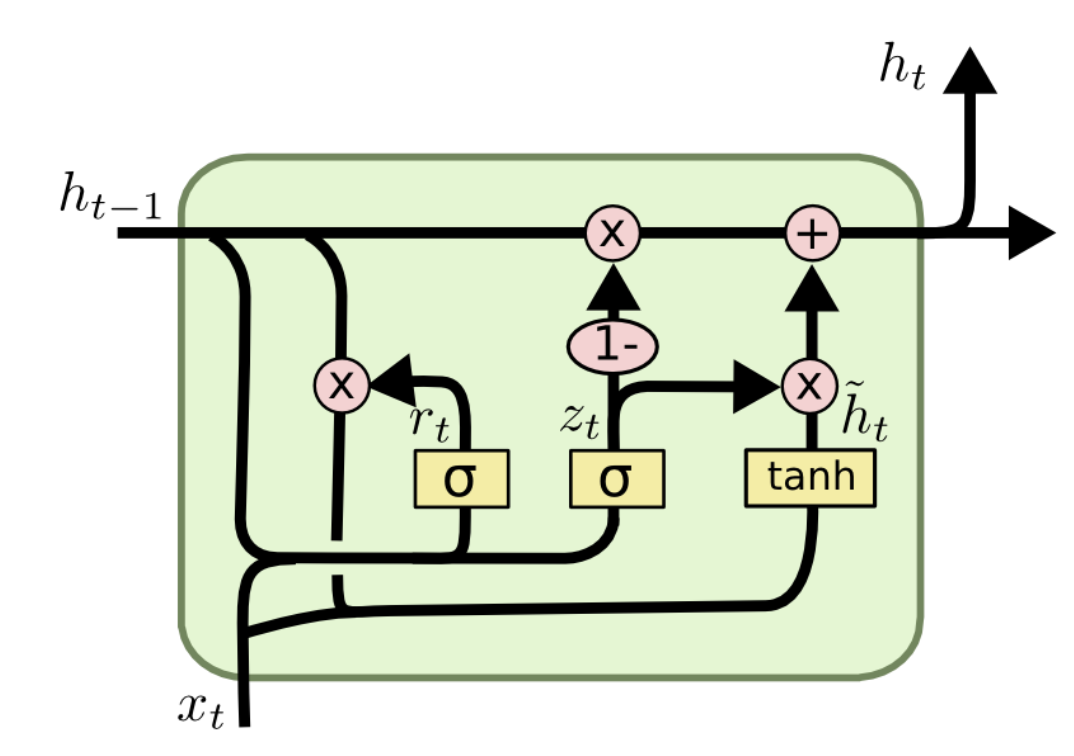
\includegraphics[width=0.5\textwidth,height=4.5cm]{lectures/06-b-rnn/image/GRU.png}
          \caption{
            Gated Recurrent Units
            \href{http://colah.github.io/posts/2015-08-Understanding-LSTMs/}{Source}
          }
          \label{fig:lstm}
\end{figure}

The update gate decides what information from the past would be passed to the next cell state.

\[z_t = \sigma(W_{zh}h_{t-1}+W_{zx}x_t + b_z) \]

The reset gate determine what information would be discarded from previous cell states.

\[r_t = \sigma(W_{rh}h_{t-1}+W_{rx}x_t + b_r) \]

Then the current memory content update the stories the latest important information by using the reset gate.

\[\widetilde{h}_t = tanh(W_{hr}(r_t*h_{t-1}) + W_{hx}x_t + b_h)\]

Finally, the final cell state updates the information gained from the current unit and passed it to the next cell.

\[h_t = (1-z_t)*h_{t-1} + z_t*\widetilde{h}_t\]